%!TEX encoding = UTF-8 Unicode
%!TEX program = xelatex

\documentclass[bachelor]{ustcthesis}
% bachelor|master|doctor
\usepackage{ustcextra}
\usepackage{pgfplots}
\usepackage{multirow}
\usepackage[position=top]{subfig}
\graphicspath{{figures/}}
%\bibliographystyle{ustcauthoryear}
\bibliographystyle{ustcnumerical}

\title{多线程并行 InSAR 数据处理\\程序的设计与实现}
\author{崔灏}
\major{固体地球物理专业}
\advisor{查显杰\ 副教授}
\submitdate{二〇一七年五月}
%\secrettext{机密\quad 小于等于20年}   % 内部|秘密|机密,注释本行则不保密
\depart{地球和空间科学学院}

\entitle{Design and implementation of multi-threaded parallel InSAR processing program}
\enauthor{CUI Hao}
\enmajor{Solid Geophysics}
\enadvisor{ZHA Xianjie, Assoc. Prof.}
\ensubmitdate{May, 2017}
%\ensecrettext{Confidential\quad Less than or equal to 20 years}  % Internal|Secret|Confidential

\begin{document}

\maketitle

%
% 本科论文:
%   frontmatter: 致谢、目录、中文摘要、英文摘要
%   mainmatter: 正文章节、参考文献
%   appendix: 附录
%
% 硕博论文:
%   frontmatter: 中文摘要、英文摘要、目录、符号说明
%   mainmatter: 正文、参考文献
%   appendix: 附录
%   backmatter: 致谢、发表论文
%

\frontmatter
\begin{abstract}

星载或机载 SAR 雷达图像是地球物理研究中常用的大地测量数据源。SAR/InSAR 成像数据处理量大、算法复杂度较高,对计算设备性能有很高的要求。然而,随着 CPU 并行计算能力的提升,在消费级个人工作站上进行 SAR/InSAR 数据处理已经成为可能。

本课题研究了以 GMTSAR 为代表的 InSAR 数据处理软件的性能瓶颈,对算法中时间复杂度较高的图像合成、图像配准模块进行了 CPU 并行优化。对真实 SAR 卫星数据的处理结果显示,对比传统串行算法,本文提出的并行算法在不降低结果精度的前提下大大提高了多核 CPU 的使用率、缩短了计算时间。

本文设计的并行算法不依赖特殊硬件,在消费级个人工作站上即可较快地完成 InSAR 数据处理,为地球物理相关科研人员提供了便利。同时,本文的思路也可以为地球物理领域的其他科学计算任务并行优化提供参考。
    
\keywords{合成孔径干涉雷达\zhspace{} 大地测量\zhspace{} 图像处理\zhspace{} 并行计算}
\end{abstract}

%\begin{enabstract}
%This is a sample document of USTC thesis \LaTeX{} template for bachelor, master
%and doctor. The template is created by zepinglee and seisman, which orignate from
%the template created by ywg@USTC\@. The template meets the equirements of USTC
%theiss writing standards.
%
%This document will show the usage of basic commands provided by \LaTeX{} and some
%features provided by the template. For more information, please refer to the
%template document ustcthesis.pdf.
%
%\enkeywords{University of Science and Technology of China (USTC), Thesis, Universal \LaTeX{} Template, Bachelor, Master, PhD}
%\end{enabstract}

\tableofcontents
\listoffigures
\listoftables
%\listofalgorithms  % 算法索引,如不需要,可直接注释掉本行
% \input{chapters/notation}

\mainmatter
\chapter{绪论}


\section{研究背景}

合成孔径雷达(synthetic aperture radar, SAR)是一种高分辨率的微波雷达成像技术。SAR 通过机载或星载微波雷达发射相干的微波信号并观察地面回波,通过信号处理得到尺度远大于雷达口径的等效“合成孔径”。SAR 成像分辨率可以达到米级,部分机载 SAR 系统甚至可以提供 10 cm 级的地表分辨率。由于 SAR 的高分辨率和全天时、全天候工作的优势,SAR 成像被广泛地用于灾害预警、遥感测绘、海洋观测、环境保护等军用和民用领域。自上世纪 80 年代以来,各国陆续发射了 ERS-1/2、Envisat、ALOS 等 SAR 卫星,星载 SAR 雷达数据成为重要的大地测量数据来源。

干涉合成孔径雷达(Interferometric SAR, InSAR)是利用多幅 SAR 图像提取高程信息的拓展应用。如果利用一组 SAR 雷达观测同一块地面区域、或者同一雷达不同时间观测同一块地面区域,由于两次观测中天线与目标相对位置存在差异(由于天线位置差异或地表形变),两幅 SAR 图像之间就会存在相位差异。相位差反映了地表高程信息或者形变信息。InSAR 成像是常用的雷达测高技术,可以取得数日到数年时间尺度上厘米级的地表形变信息,被广泛地用于地震、地面沉降、固体潮等长短周期的地表形变观测。

SAR/InSAR 成像算法是一个复杂的信号处理过程。典型的 SAR 成像算法如距离多普勒算法,它包括距离向压缩(range compression)、距离向徙动校正(range migration)和方位向压缩(azimuth compressions)三个基本步骤。信号压缩通过匹配滤波实现,可以借助快速傅立叶变换算法在频域高效实现。SAR 数据处理技术已经比较成熟,可以通过数字信号处理器高效地实现。包括日本 ALOS 在内的许多 SAR 数据源直接向终端用户提供了 SAR 成像处理后的单视复图像(single look complex,SLC)。因此,对于地球物理研究工作等终端应用,往往不需要接触 SAR 成像算法,直接对获取的 SLC 图像进行 InSAR 成像即可。

InSAR 成像算法时间和空间复杂度比较高。在大地测量领域,InSAR 成像范围宽度可达数百公里,成像数据量十分巨大,这对成像程序的性能提出了很高要求。科研工作者通常使用个人电脑或服务器 CPU 进行 InSAR 数据处理,这类桌面平台上常用的 SAR/InSAR 数据处理软件有 GMTSAR、ISCE(InSAR Scientific Computing Environment)等。

近年来,桌面中央处理器(Central Processing Unit, CPU)主频受制于物理极限已趋于饱和,厂商开始发展多核心 CPU 技术,提高 CPU 并行处理能力。近几年的消费级个人电脑往往都已经配备具有 4 到 8 个中央处理单元的多核心 CPU;服务器甚至可能配置多个多核心 CPU,达到数十个逻辑计算核心。但无论是个人电脑还是服务器,乃至具有312万个计算核心的天河二号超级计算机,其单任务处理能力仍是十分有限(CPU 主频一般在 1GHz 到 4GHz)。只有运行多个计算任务、或者运行专门设计的并行处理程序,才能充分发挥多核心的并行优势。

以 GMTSAR 为代表的传统串行 InSAR 处理软件无法发挥多核心 CPU 的并行处理能力,计算能力仍受制于单核心计算性能。为了满足大地测量中大规模 InSAR 数据处理的需求,本课题对 GMTSAR 的 InSAR 处理算法的部分重要模块进行了并行优化,以期在桌面多核心 CPU 平台上减少数据处理时间。

\section{现有工作}

现在,InSAR 成像算法已经比较成熟,主要包括图像配准、干涉相位合成、相位滤波和相位解缠等基本模块。加州大学圣迭戈分校(UC San Diego)和斯克里普斯海洋研究所(Scripps Institution of Oceanography)开发的 SAR/InSAR 处理软件 GMTSAR 是学习 InSAR 成像算法的重要范本。GMTSAR 仅能使用 CPU 单线程进行 InSAR 成像,计算效率不高。但由于其源代码完全开放,任何人都可以免费获取并自由修改,因此在地球物理学术界应用非常广泛。

目前已经有一些针对特定硬件优化 InSAR 算法的实例。\citet{shayu2014} 在多核数字信号处理器(Digital Signal Process, DSP)上实现了实时 InSAR 数据处理,并探讨了在现场可编程逻辑门阵列(Field Programmable Gate Array, FPGA)硬件上实现高效并行 InSAR 数据处理的可行性。这类多核 DSP 芯片和 FPGA 设备具有低功耗和良好的并行性,适合在嵌入式设备上使用,比如可以整合进 SAR 雷达系统。但在桌面平台,这类特殊硬件非常少见。

图形处理器(Graphics Processing Unit, GPU)是另一类具有强大并行处理能力的微处理器,并且往往具有较大的独立内存空间(显存)。\citet{reza2015accelerating} 在 NVIDIA GPU 上借助 CUDA 通用计算框架实现了高效的相位解缠算法,对比 CPU 程序取得了数十倍的性能提升,并显著降低了计算功耗。未来,基于 GPU 的通用计算有望成为高性能计算应用的主要平台。但目前 GPU 通用计算技术还在发展阶段,在科学计算领域应用并不广泛。

\section{课题内容简介}

本课题基于 GMTSAR 公开的 InSAR 成像算法,选取图像配准(image alignment)和图像拼接两个计算复杂度比较高的程序模块,设计并实现了多 CPU 并行处理算法,以期在桌面或服务器多核心 CPU 上改善 InSAR 成像程序的性能。本文详细介绍了两个并行处理算法的设计方案,并简要探讨了其他 InSAR 数据处理模块的并行优化思路。

在公开的 ALOS 卫星数据上进行的测试显示,CPU 并行处理算法在不降低结果精度的条件下显著提高了多核心 CPU 平台上 InSAR 数据处理的效率。本文给出了并行算法与 GMTSAR 串行算法的性能比较数据,并定性地分析了性能提升的来源。


\chapter{算法设计和优化}

\section{InSAR 成像算法简介}

\subsection{InSAR 测高原理}

讨论并行 InSAR 数据处理算法前,先对 InSAR 成像原理做一个简单介绍。\cite{simons2007interferometric} \cite{ferretti2007insar}

\begin{figure}[ht]
\centering
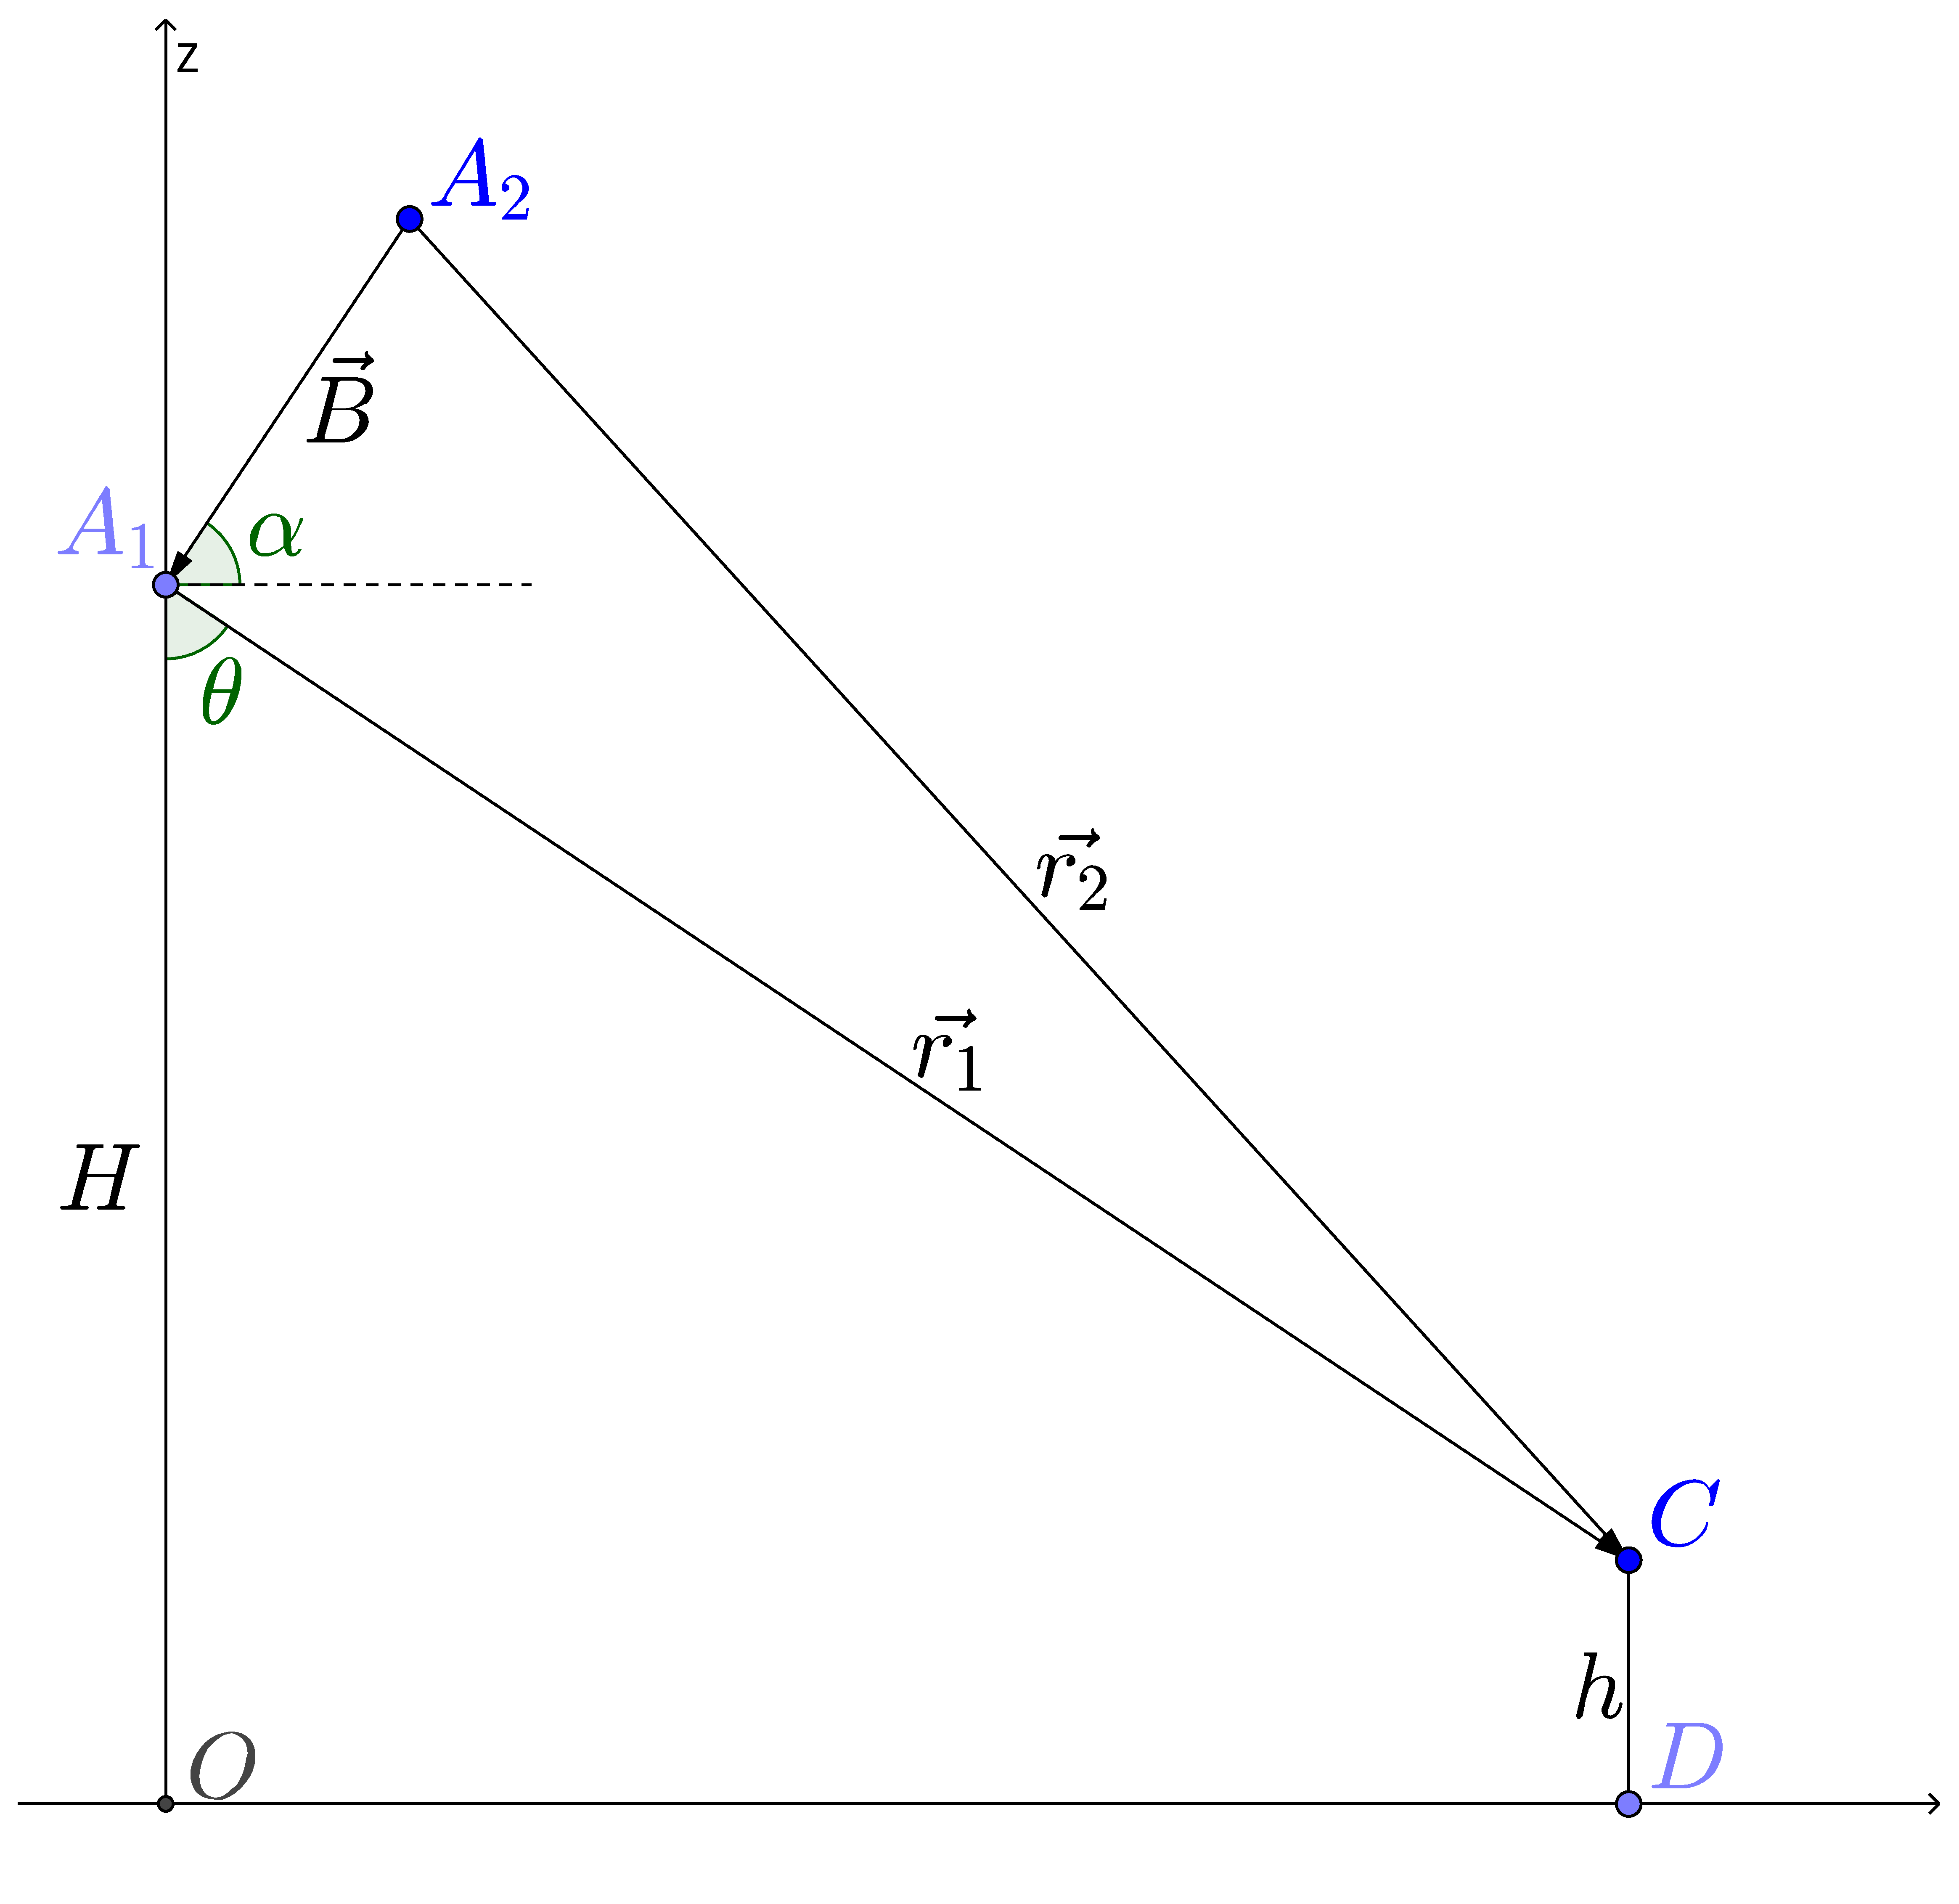
\includegraphics[width=0.4\textwidth]{insar_simple}
\caption{InSAR 高程测量基本原理} \label{fig:insar_simple}
\end{figure}

图 \ref{fig:insar_simple} 展示了利用两个 SAR 雷达观测同一地面单位进行 InSAR 测高的基本原理。InSAR 测量地表形变的原理与之类似。$A_1$ 和 $A_2$ 表示主天线和副天线位置,两天线空间位移矢量为 $\vec{B}$,称为 InSAR 基线,角度 $\alpha$ 为基线与水平面夹角。$C$ 为地面目标点,相对于两天线的位移矢量分别为 $\vec{r_1}$ 和 $\vec{r_2}$,称为斜距。角度 $\theta$ 为主天线观察方向与竖直方向的夹角,称为下视角。

斜距矢量 $ \vec{r_1} $ 和 $ \vec{r_2} $ 可以根据天线方向和微波信号双程旅行时得到。雷达位置或 SAR 卫星轨道,即基线 $\vec{B}$ 和天线高度 $H$,也可以认为是已知的。

由简单的几何关系可知,目标点高度可以表示为:

\begin{equation}
    h = H - r_1 \cos\theta
\end{equation}

为了得到 $\theta$,分别从主天线和副天线取得对焦后的 SAR 图像。该图像具有复数像素值,包含从单一视角观测的回波幅度和相位信息(即目标点的散射系数),因此称为单视复图像(Single Look Complex,SLC)。SLC 图像像素基本对应于 SAR 雷达最小分辨区域,对于星载设备可达数十米量级\cite{sandwell2011gmtsar})。

目标点 $C$ 在主、副 SLC 图像上的复像素值 $P_1$ 和 $P_2$ 可以表示为:

\begin{equation}
\begin{split}
    P_1(\vec{r_1}) = A_1(\vec{r_1}) \exp(i \frac{4\pi}{\lambda} r_1) \\
    P_2(\vec{r_2}) = A_2(\vec{r_2}) \exp(i \frac{4\pi}{\lambda} r_2) \\
\end{split}
\end{equation}

将两幅 SLC 图像共轭相乘,即得到一幅干涉图像:

\begin{equation}
    P_{\textrm{int}} = P_1^* P_2 =  A_1 A_2 \exp(i \frac{4\pi}{\lambda}(r_2 - r_1))
\end{equation}

干涉图相位项中的 $ r_2 - r_1 $ 可以通过余弦定理展开:
\begin{equation}
\begin{split}
    r_2 - r_1 &= r_1 (\frac{r_2}{r_1} - 1) \\
              &= r_1 \sqrt{1- \frac{\vec{r_1} \cdot \vec{B}}{r_1} + (\frac{B}{r_1})^2}
\end{split}
\end{equation}

基线长度 $B$ 一般远小于斜距 $r_1$、$r_2$,上式可以简化为:
\begin{equation}
    r_2 - r_1 = - \vec{r_1} \cdot \vec{B} = - r_1 B \cos(\frac{\pi}{2} - \theta + \alpha)
\end{equation}

故 $\theta$ 可以通过干涉图相位求出,进而得到目标点高程 $h$。实际上回波相位总是折叠到一个 $2\pi$ 周期内的,因此干涉图相位也折叠在一个 $2\pi$ 周期中,这称为相位缠绕(phase wrap)。连续的相位值仍可以通过相位解缠算法估计出来。

实际的 SAR 雷达工作高度 $H$ 可达数十到数百千米,如 ALOS 卫星工作轨道高度为 700km\cite{web:alos},因此必须考虑地球曲率的影响。研究地表形变或位移时,原始地形引起的相位差也要通过数字高程模型去除。此外,轨道偏移、电离层噪声、对流层噪声等因素也对相位测量造成干扰。

\subsection{InSAR 成像算法}

虽然 InSAR 测高原理非常简单,但实际的成像算法要复杂得多。主要可以归纳为以下若干步骤\cite{sandwell2011gmtsar}:

\textbf{SAR 成像和预处理}:相位差的测量精度决定了 InSAR 测高的精度。进行干涉的两幅 SAR SLC 图像必须对成像区域有较好的聚焦,并且具有合适的基线长度,需要在若干组 SAR 数据中进行\textbf{筛选}。为了提取成像区域的有效信息,往往需要对 SAR 数据进行\textbf{拼接}或\textbf{切割}。

\textbf{图像配准}(image registration):因天线视角、轨道偏移等因素,主、副 SLC 图像成像区域往往有一定差异。进行干涉成像之前,要通过图像配准将副 SLC 图像映射到和主 SLC 图像同样的成像区域。图像配准是 InSAR 数据处理中计算复杂度较高的一个步骤。

\textbf{干涉成像}:将对齐的主、副 SAR SLC 图像进行共轭相乘,得到干涉图像。干涉图相位信息反映了地面高程或地表位移信息,但被折叠到一个 $2\pi$ 周期上。

\textbf{相位修正}:根据研究对象的不同,从干涉图中可选地去除地形相位、电离层延迟等不需要的相位项,以及滤除各种影响结果精度的噪声。

\textbf{相位解缠}:利用高程或形变的连续性,从折叠相位恢复出连续变化的相位,以在较大的尺度上反映高程或形变信息。相位解缠是 InSAR 数据处理中技巧性比较高的一个步骤。

上述步骤即为 InSAR 数据处理程序的主要功能。除此之外,包括 GMTSAR 在内的 InSAR 处理软件还包含很多其他辅助分析模块,研究人员可以查阅相关文档以进一步了解。


\section{CPU 多线程并行算法设计}

本节将以 GMTSAR 中图像拼接预处理和相位解缠两个程序模块为例子,介绍 CPU 并行的 InSAR 成像程序的算法设计和具体实现。

\subsection{并行图像配准算法}

InSAR 干涉成像要求输入的主、副 SAR SLC 图像精确对应同样的成像区域,以确保干涉图的相干性。但由于轨道偏移、天线视角、采样率变化(由天线移动速度差异或工作参数变化导致)等因素,副 SLC 图像成像区域相对主 SLC 图像成像区域会发生位移、旋转、拉伸等类型的畸变。图像配准的目的是找到主、副 SLC 图像坐标间的映射关系,以消除这些畸变。

在各类导致图像偏移的因素中,轨道偏移和雷达视角差异是主要的影响因素。这部分偏移可以通过精确的 SAR 天线轨道数据与工作状态计算出。\citet{sandwell2011gmtsar} 指出,对于 ALOS 等星载 SAR 雷达,基于精确轨道数据计算的偏移量在方位向精度为大约2像素、距离向大约1像素。但 InSAR 成像往往要求达到至少 1/10 像素的配准精度 \cite{li2008image},因此除了利用已知的轨道参数进行\textbf{粗配准},还必须利用两幅图像本身的相关性进行\textbf{精配准}。

图像配准的精确性一般通过配准后图像的\textbf{相干性}(coherence)进行评估。对于两幅 SLC 图像 $P_1$ 和 $P_2$,在像素 $(x, y)$ 周围某个采样区域 $D(x, y)$ 上的相干性 $\gamma(x, y)$ 定义为 \footnote{本文使用变量或下标 $x$ 代表方位向坐标或相关量,使用变量或下标 $y$ 代表距离向相关量。}:

\begin{equation}
    \gamma(x, y) = \frac{\sum_{x', y'} P_1(x', y') P_2^*(x', y')}{\sqrt{\sum_{x', y'}|P_1(x', y')|^2 \sum_{x', y'}|P_2(x', y')|^2}} \qquad (x', y') \in D(x, y)
    \label{eq:coherence}
\end{equation}

GMTSAR 中的 xcorr 和 fitoffset.csh 程序实现了图像配准,它将主 SAR SLC 图像像素到副 SLC 图像之间的映射近似为一个二维仿射变换。即副 SLC 图像上的坐标 $(x_i', y_i')$ 与主 SLC 图像坐标 $(x_i, y_i)$ 通过6个仿射变换参数相联系:

\begin{equation}
\begin{bmatrix}
  t_i x_i' \\
  t_i y_i' \\
  t_i \\
\end{bmatrix}
= \begin{bmatrix}
       a & b & c \\
       d & e & f \\
       0 & 0 & 1 \\
\end{bmatrix}
\begin{bmatrix}
  x \\
  y \\
  1 \\
\end{bmatrix}
\end{equation}

如图 \ref{fig:register} 所示,xcorr 从主 SLC 图像中等间隔选取 $n_x \times n_y $ 个大小为 $w_x \times w_y$ 的采样位置 $(x_c, y_c)_{i,j}$($0 \leq j < n_x$,$0 \leq i < n_y$)。每个采样位置映射到副 SLC 图像中的坐标 $(x'_c, y'_c)_{i,j}$,偏移量可以看作在粗配准偏移矢量 $(\Delta_x, \Delta_y)$ 的基础上加上一个局部修正项 $(\delta_x, \delta_y)_{i,j}$,即:

\begin{equation}
    (x'_c, y'_c)_{i,j} = (x_c, y_c)_{i,j} + (\Delta_x, \Delta_y) + (\delta_x, \delta_y)_{i,j}
\end{equation}

\begin{figure}[htbp]
\centering
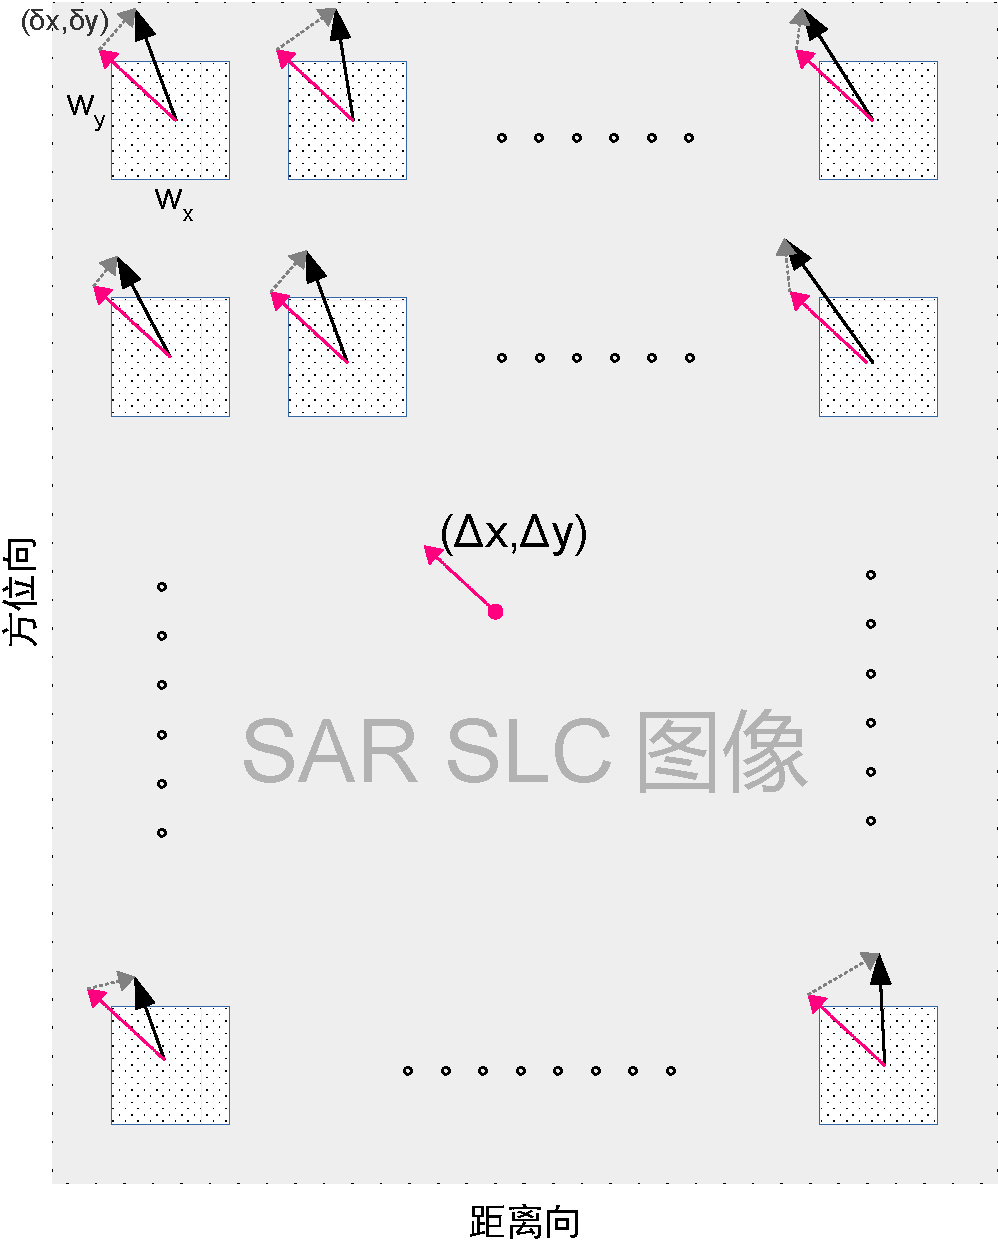
\includegraphics[width=0.6\textwidth]{register}
\caption{GMTSAR xcorr 配准算法示意} \label{fig:register}
\end{figure}

如前文所述,$\Delta_x$、$\Delta_y$ 已经可以提供几个像素的配准精度,因此可以在一个较小的采样窗口中搜索 $(\delta_x, \delta_y)$(xcorr 默认采样窗口大小 $w_x \times w_y = 64 \times 64$)。xcorr 通过局部搜索(散射系数幅度)的互相关最大值来判断修正项的大小。即,对于主 SLC 图像中以 $(x_c, y_c)$ 为中心的采样窗口 $D_1$ 和副 SLC 图像中以 $(x_c + \Delta_x, y_c + \Delta_y)$ 为中心的采样窗口 $D_2$,计算出互相关矩阵 $D_1 \star D_2$,局部的偏移矢量修正项 $(\delta_x, \delta_y)$ 满足:

\begin{equation}
    (D_1 \star D_2)[\delta_x, \delta_y] = \max(D_1 \star D_2)
\end{equation}

得到各个采样位置的精配准偏移量后,fitoffset.csh 选取其中互相关性较好的数据,通过最小二乘法拟合出6个仿射变换参数。

搜索互相关矩阵至多达到到1个像素的配准精度。为了得到次像素级精度的偏移矢量,需要对原始数据或互相关矩阵进行插值处理。目前并没有一个公认有效的插值方法,不同论文选择的插值算法、插值顺序都有所区别\cite{li2008image}\cite{hanssen1999evaluation}。对于每个采样窗口,xcorr 在计算互相关矩阵前后分别进行了两次 sinc 插值(具体算法流程如图 \ref{fig:xcorr} 所示):

\textbf{原始采样窗口像素的距离向插值}:如前文所述,粗配准精度在距离向上比方位向上更差一些。为了补偿这一精度差异,xcorr 计算互相关矩阵前在距离向对采样窗口像素进行 sinc 插值。sinc 插值可以通过 FFT 和频域补0高效地实现。插值因子默认 $\iota_r = 2$。

\textbf{互相关矩阵插值}:对互相关矩阵进行插值是获得次像素精度偏移矢量的常用方法,一般采用线性插值、sinc 插值或者样条插值方法\cite{hanssen1999evaluation}。这一步 xcorr 使用的仍是 sinc 插值,插值在方位向和距离向都要进行,默认插值因子 $\iota_x = \iota_y = 16$。

图 \ref{fig:xcorr} 的局部配准算法仍有改进空间。前述图像配准算法只用到 SLC 图像幅度信息。除了距离向插值要使用复序列 FFT 对原始序列进行处理,后面的算法流程实际上已经抛弃了相位信息,因此使用实序列 FFT 算法(FFT of real data,RFFT)处理采样窗口和互相关矩阵即可。处理实序列时,RFFT 比复序列 FFT 节省一半的运行时间和存储空间。改进后的局部配准流程如图 \ref{fig:xcorr2} 所示。

\begin{figure}[htbp]
\centering
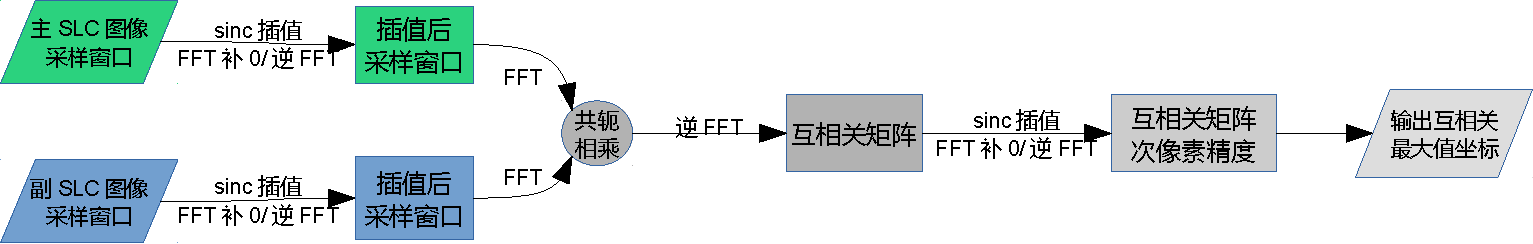
\includegraphics[width=0.99\textwidth]{xcorr-crop}
\caption{GMTSAR xcorr 局部配准算法流程} \label{fig:xcorr}
\end{figure}

\begin{figure}[htbp]
\centering
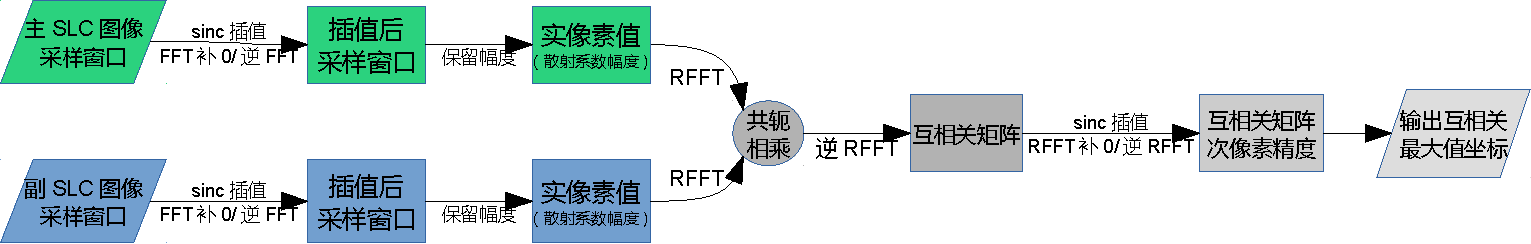
\includegraphics[width=0.99\textwidth]{xcorr2-crop}
\caption{改进的局部配准算法流程}
\note{部分复序列 FFT 算法改成了实序列 FFT 算法(RFFT)}
\label{fig:xcorr2}
\end{figure}

本课题基于上述图像配准算法,设计了多线程并行 SLC 图像配准程序 xcorr2。为了理解 xcorr2 的并行设计,首先要从计算复杂度、内存占用、文件读取三个角度定性分析并行算法的预期性能指标:

\begin{itemize}
    \item \textbf{计算时间}:对于默认 $64 \times 64 = 4096$ 点的采样窗口,现代桌面 CPU 完成单线程复序列 FFT 计算的时间大约在几 ms 到 50ms 的数量级\cite{fftwbench}。图 \ref{fig:xcorr2} 所示的局部配准需要4次复序列 FFT 或逆 FFT,5次 RFFT 或逆 RFFT,以及一次实复矩阵(逐元素)乘法。以默认参数完成整幅图像配准需要遍历 512 个采样窗口。作为一个简单的估计,完成一次配准需要的 CPU 单线程计算时间约为 10~100s。
    \item \textbf{内存占用}:SAR SLC 图像文件大小可达数GB,但配准过程只需要读取采样窗口的数据。虽然采样窗口默认大小只有 $4096$ 个数据点,但插值后的互相关矩阵可达 $1024^2 = 1M$ 个数据点。考虑到计算过程要存储若干次中间结果,包括 FFT 变换结果、插值序列和互相关矩阵等,将数据点的数量乘以10作为估计值,即需要存储约 10M 个数据点,则可以估计每次局部配准过程需要的内存空间约为数十 MB。并行算法会增加内存开销(正比于计算线程数量),但相对于桌面工作站典型的 4~16GB 的内存配置,预期的内存占用并不大。
    \item \textbf{文件读取延迟}:典型的机械硬盘由于磁头寻道产生的延迟则至少在 10ms 的量级\cite{wiki:hddcharacter},相比于 FFT 计算时间仍是不可忽略的。考虑使用单独的线程进行文件读取,并使用更多的内存预存 SLC 数据。
\end{itemize}

\begin{figure}[ht]
\centering
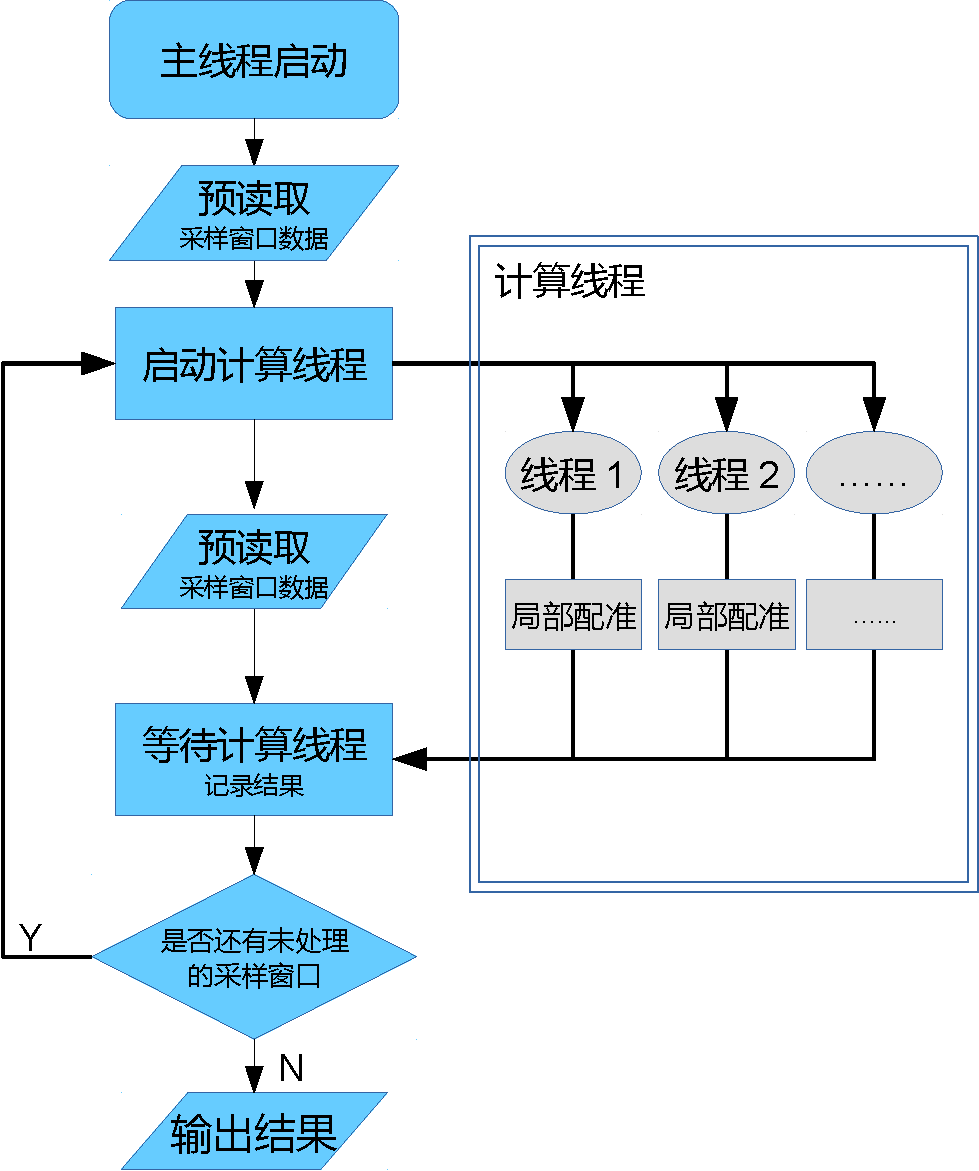
\includegraphics[width=0.6\textwidth]{parallel}
\caption{xcorr2 并行图像配准程序多线程架构} \label{fig:parallel}
\end{figure}

综合上述因素,xcorr2 使用了如图\ref{fig:parallel}所示的主-副多线程并行架构。这一设计的核心是用独立的\textbf{主线程}进行数据预读取,而线程池中的\textbf{计算线程}则负责进行局部配准算法。单线程文件读取可以充分发挥机械硬盘顺序读写的优势,避免多线程磁盘读写(IO)相互竞争影响性能。内存开销方面,主线程每次只提前多读取一组待处理的采样窗口数据,并行内存开销相当于 单线程内存开销 $\times$ 线程数 $\times 2$。

理想情况下,主线程 IO 操作与计算线程局部配准任务完全并行,并且文件读取不慢于一次局部配准所需的时间(按照前面的分析应当是成立的),则并行算法的加速比\footnote{加速比:串行算法计算时间与相应并行算法计算时间之比。}应当正比于计算线程数量。

\subsection{基于并行规约的图像拼接算法}

图像拼接是 InSAR 数据处理中常见的预处理或后期处理操作。为了得到较大区域的 InSAR 图像,通常可以采用两种图像拼接方法。两种拼接方法的差异仅仅是操作数据的不同,因此本文将合并讨论:

\begin{itemize}
    \item \textbf{SAR 图像帧拼接}:包括 ERS、InSAR 在内的 SAR 卫星,用轨道号(track)和图像帧号(frame)标记不同时间和观测位置的 SAR 数据。同一轨道号的连续图像帧对应的观测区域是在方位向连续的,分成若干帧以便于存储和分发。大地测量应用中,成像范围可能包含多个图像帧,因此要将帧号连续的 SAR 数据文件或者 SLC 图像依次合并,以得到较大的成像区域。GMTSAR 中的 ALOS\_Merge 程序模块用于进行 ALOS 卫星数据的拼接。
    \item \textbf{InSAR 干涉图拼接}:除了合并 SAR 数据,也可以分区域进行 InSAR 成像后再进行图像拼接。因为跨轨道号的 SAR 数据没有成像区域上的连续性,要得到距离向跨多个图像帧的干涉图像,只能在 InSAR 成像后进行拼接。虽然 GMTSAR 没有直接提供拼接程序,但会以 NetCDF 4 文件格式导出相位解缠后的 InSAR 干涉图,该格式可以很方便地使用 Python、Matlab 等编程语言读取和合并。
\end{itemize}

除了 SAR/InSAR 数据处理中的应用,文件拼接也是科研数据处理中常见的操作。数据文件往往受存储器或通信方式的限制,必须分块存储,而在数据处理时要重新合并成连续的数据文件。这类拼接操作的原始数据是串行生成的,其编号反映了时间或者空间位置上的顺序,因此合并时必须保持特定的拼接的顺序。文件拼接操作 $\oplus$ 满足结合性,但不满足交换性:

\begin{equation}
\begin{split}
    (F_i \oplus F_j) \oplus F_k = F_i \oplus (F_j \oplus F_k) \qquad &\forall F_i, F_j, F_k \in \textrm{\{data files\}} \\
    F_i \oplus F_j \neq F_j \oplus F_i \qquad &\exists F_i, F_j \in \textrm{\{data files\}}
\end{split}
\end{equation}

\begin{figure}[htbp]
\centering
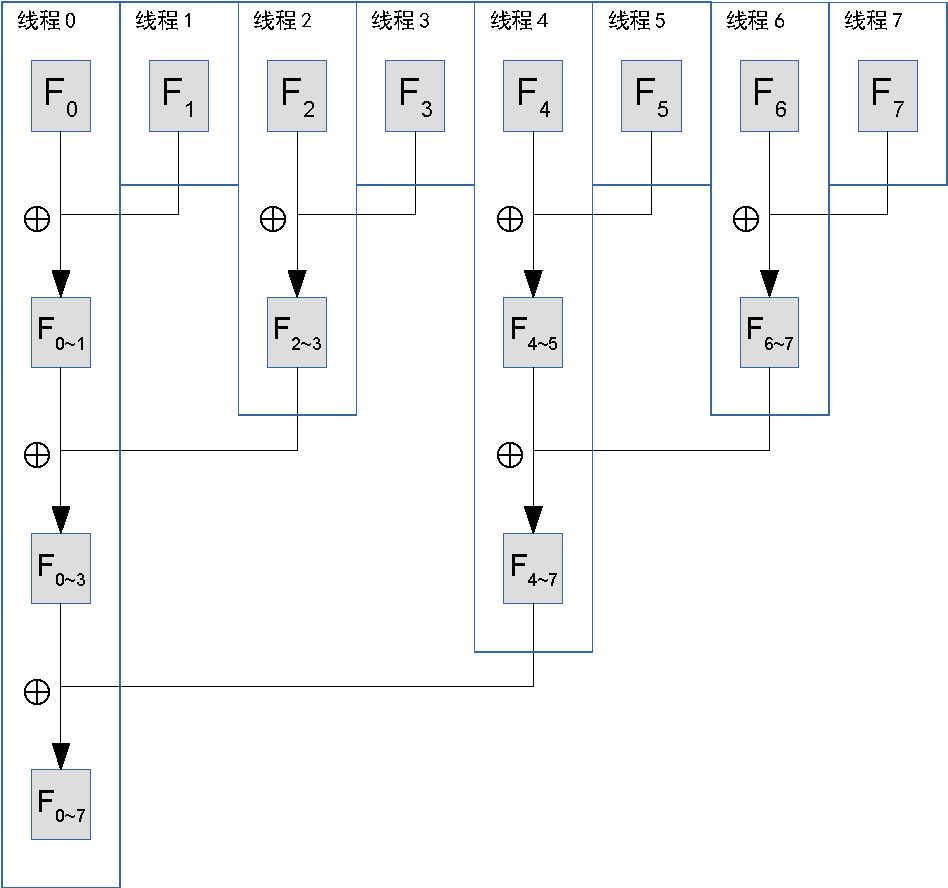
\includegraphics[width=0.8\textwidth]{reduce-crop}
\caption{基于并行规约的图像拼接算法流程示意} \label{fig:reduce}
\end{figure}

文件拼接的顺序要求为程序并行化带来了挑战。这类合并算法,仍可以利用结合性改造为并行算法,这种技术称为并行规约(reduce)\cite{chen2002paraalgo}。图 \ref{fig:reduce} 展示了并行规约技术的工作流程。规约技术将串行的拼接操作分解为连续的文件序列上的拼接操作,完成一轮拼接后,再通过下一轮迭代将上一轮生成的结果分组拼接,不断迭代直至完成整个文件序列的拼接。并行规约图像拼接算法可以非常简洁地通过程序实现。程序伪代码如图 \ref{fig:reduce-algo} 所示。

\begin{figure}[htbp]
\begin{lstlisting}[language=C]
// threadId: 线程编号
// 全部线程结束后,文件 0 为拼接后的结果
void mergingThread(int threadId) {
    int level = 1;

    while (threadId & level != 0)
        int another = threadId + (1 << level);

        waitThread(another);  // 等待编号为 another 的线程

        // 将编号为 another 的文件合并进编号为 current 的文件
        mergeTwoFile(current, another);
        
        level = level * 2 + 1;
    }

    terminateThread();  // 停止当前线程
}
\end{lstlisting}
\caption{基于并行规约的图像拼接算法伪代码示意}
\label{fig:reduce-algo}
\end{figure}

可以看到,并行规约的图像拼接算法中各工作线程的工作量是不平均的,算法最后会收敛为单线程执行。当要拼接的文件数量较多时可以较好发挥多核心 CPU 的并行计算优势。

理论上,如果忽略文件大小对拼接效率的影响,并且不考虑有效并行线程数的限制,规约技术可以将操作时间从大约 $N \times t$(t 为合并一对文件耗费的时间)缩短至 $\log_2(N) \times t$。

\subsection{其他程序模块的并行优化分析}

InSAR 数据处理是一个复杂计算过程,整个 GMTSAR 软件包含大量 SAR/InSAR 数据处理和辅助分析程序模块。受时间和个人能力所限,本课题无法对整个 GMTSAR 软件进行分析和优化。但值得注意的是,前文所提出的优化方案也应当可以推广到其他程序模块上。本节再通过两个例子说明这一点。

\textbf{干涉图生成模块}(GMTSAR 中的 phasediff 程序)是 InSAR 成像技术的核心,但基本算法并不复杂,只需要简单地计算已经配准的主、副 SLC 图像的相位差、并移除地球曲率造成的相位项即可。对此可以利用与并行图像配准算法同样的思路,将图像分块交给多个线程并行处理。

\textbf{相位解缠模块}(GMTSAR 中的 snaphu 程序)使用 \citet{chen2002phase} 提出的统计耗费网络流算法(Statistical-cost Network-flow algorithm for Phase Unrapping, SNAPHU)进行相位解缠。该算法将解缠相位微分畸变最小化问题转换为最小费用流问题,使用图论中的 Prim 算法和 Dijkstra 算法搜寻相邻的残点\cite{cheng2007insar}。Prim 算法和 Dijkstra 算法的核心均为广度优先搜索,即从单点向相邻的所有点扩展搜索出一个最优结果。广度优先搜索问题一般都可以通过规约技术实现并行。此外,SNAPHU 算法可以对较大的图像进行分片处理,各分片之间没有数据相关性,因此也可以很方便地以分片为单位并行处理。

此外,多计算任务简单并行也是一种常用的优化手段,即同时运行若干程序实例处理不同的输入数据。虽然这种并行粒度粗,执行小规模计算任务时往往不能实现,但在某些场景下仍可能是最为简单有效的方案。

\chapter{实验测试与分析}

本节使用的 InSAR 测试数据是 GMTSAR 官方提供的2010年4月下加利福尼亚州 $7.2 M_w$ 地震前后的 ALOS 卫星数据。主、副 SAR SLC 图像分别拍摄于2009年12月17日和2010年5月4日。SLC 图像大小为一个标准的 ALOS 图像帧,方位向和距离向长度各为 27648 像素和 11304 像素。软件测试环境如表 \ref{tab:env} 所示。

\begin{table}[htbp]
\centering
\begin{tabular}{|l|l|l|}
\hline
    \multirow{3}{*}{CPU}                        & 型号     & Intel Xeon E5-2650 v4                 \\ \cline{2-3} 
                                                & 核心数   & $\times 12$                           \\ \cline{2-3} 
                                                & 主频     & 2.20 GHz                              \\ \hline
    \multicolumn{2}{|l|}{内存}                             & 32768 MiB                             \\ \hline
    \multicolumn{2}{|l|}{操作系统}                         & Ubuntu 16.04.2 LTS, Linux 4.4.0 内核  \\ \hline
    \multicolumn{1}{|c|}{\multirow{2}{*}{编译}} & 编译器   & gcc 5.4.0                             \\ \cline{2-3} 
    \multicolumn{1}{|c|}{}                      & 编译参数 & \texttt{-O2 -march=native}            \\ \hline
\end{tabular}
\caption{软件测试环境} \label{tab:env}
\end{table}

\section{图像拼接算法测试}

并行图像拼接算法的实验测试中,因为数据来源有限,仅仅使用了6个同一轨道号的连续的 SAR 图像帧进行测试。图 \ref{fig:exp_merge} 展示了并行线程数对拼接程序性能的影响。可以看到,并行归约算法将拼接时间缩短了一半以上。比较遗憾的是,由于要拼接的图像帧数量较少,归约算法的线程数很快就收敛了,并行算法性能大概在2~3个线程时就达到了饱和。

\begin{figure}[htbp]
\centering
\subfloat[程序计算时间]{
    \label{fig:exp_merge_a}
    \begin{minipage}[t]{0.49\textwidth}
        \centering
        \resizebox {\textwidth} {!} {
            \begin{tikzpicture}
\begin{axis}[
    xlabel={并行线程数},
    ylabel={计算时间/s},
    xmin=1, xmax=7,
    ymin=0, ymax=200,
    xtick={1, 2, 3, 4, 5, 6, 7},
%    ytick={ },
    legend pos=north east,
    ymajorgrids=true,
    grid style=dashed,
]

\addplot[
    color=red,
    mark=square,
    style=solid,
    ]
    coordinates {
        (1, 194.972254756)
        (2, 106.441216719)
        (3, 91.799094679)
        (4, 92.142388643)
        (5, 92.000214744)
        (6, 88.829891908)
        (7, 83.641275544)
    };
\end{axis}
\end{tikzpicture}

        }
    \end{minipage}
}
\subfloat[CPU 核心利用率]{
    \label{fig:exp_merge_b}
    \begin{minipage}[t]{0.49\textwidth}
        \centering
        \resizebox {\textwidth} {!} {
            \begin{tikzpicture}
\begin{axis}[
    xlabel={并行线程数},
    ylabel={CPU 核心占用},
    xmin=1, xmax=7,
    ymin=0, ymax=4,
    xtick={1, 2, 3, 4, 5, 6, 7},
%    ytick={ },
    legend pos=north east,
    ymajorgrids=true,
    grid style=dashed,
]

\addplot[
    color=red,
    mark=square,
    style=solid,
    ]
    coordinates {
        (1, 1.000)
        (2, 1.862)
        (3, 2.257)
        (4, 2.258)
        (5, 2.298)
        (6, 2.425)
        (7, 2.575)
    };
\end{axis}
\end{tikzpicture}

        }
    \end{minipage}
}
\caption{线程数对 SAR 图像帧并行拼接算法性能的影响} \label{fig:exp_merge}
\note{\small 测试数据共6个 ALOS 图像帧}
\end{figure}
 
该例子说明,并行算法的性能并非总是随着线程数的增加而提升。计算线程数量超过一定值后,多余的线程将不会改善程序性能,必须改进算法或者提高数据量以增加可利用的线程数。此外,线程数量增加时,线程间通信的成本会增加,其他不可并行资源访问(如磁盘读写)也可能达到性能瓶颈。

图像拼接算法完全是确定性的,不会受拼接顺序影响。经过验证。并行拼接与顺序拼接的结果完全一致。

\section{图像配准算法测试}

图 \ref{fig:exp_cores} 展示了默认计算参数(见表 \ref{tab:xcorr-args})下 xcorr2 性能随计算线程数的变化趋势。当计算线程从无增加至6个时,图 \ref{fig:exp_cores_a} 显示的计算时间缩短非常显著。但当计算线程数进一步增加时,运行时间并没有显著变化。图 \ref{fig:exp_cores_b} 中的 CPU 核心使用率也反应了这种趋势,当计算线程数多于6个时,核心使用率少于计算线程数,说明程序已经无法充分利用所有的 CPU 核心。后面的实验中将使用8个计算线程对 xcorr2 并行性能进行评估,

\begin{figure}[htbp]
\centering
\subfloat[程序计算时间]{
    \label{fig:exp_cores_a}
    \begin{minipage}[t]{0.49\textwidth}
        \centering
        \resizebox {\textwidth} {!} {
            \begin{tikzpicture}
\begin{axis}[
    xlabel={计算线程数},
    ylabel={计算时间/s},
    xmin=0, xmax=12.2,
    ymin=0, ymax=12,
    xtick={0, 2, 4, 6, 8, 10, 12},
%    ytick={ },
    legend pos=north east,
    ymajorgrids=true,
    grid style=dashed,
]
\addplot[
    color=blue,
    mark=square,
    ]
    coordinates {
        (0, 11.200907922)
        (1, 10.521500231)
        (2, 5.431319614)
        (3, 3.757715043)
        (4, 2.918596810)
        (6, 2.146015373)
        (8, 2.052885075)
        (12, 2.181156634)
    };
    \legend{xcorr2} 
\end{axis}
\end{tikzpicture}

        }
    \end{minipage}
}
\subfloat[CPU 核心利用率]{
    \label{fig:exp_cores_b}
    \begin{minipage}[t]{0.49\textwidth}
        \centering
        \resizebox {\textwidth} {!} {
            \begin{tikzpicture}
\begin{axis}[
    xlabel={计算线程数},
    ylabel={占用 CPU 核心数},
    xmin=0, xmax=12.2,
    ymin=0, ymax=10,
    xtick={0, 2, 4, 6, 8, 10, 12},
%    ytick={ },
    legend pos=north west,
    ymajorgrids=true,
    grid style=dashed,
]

\addplot[
    color=red,
    mark=square,
    style=solid,
    ]
    coordinates {
        (12,8.667)
        (8 ,7.296)
        (6 ,6.414)
        (4 ,4.438)
        (3 ,3.376)
        (2 ,2.304)
        (1 ,1.168)
        (0 ,1.000)
    };
    \legend{xcorr2}
\end{axis}
\end{tikzpicture}

        }
    \end{minipage}
}
\caption{使用不同数量计算线程对 xcorr2 配准性能的影响}
\note{xcorr2 运行时会启动一个主线程和若干计算线程,主线程不参与计算。计算线程数为0代表不启动计算线程,直接使用主线程串行计算。}
\label{fig:exp_cores}
\end{figure}

\begin{table}[htbp]
\centering
\begin{tabular}{|l|l|l|}
    \hline
    \textbf{参数} & \textbf{符号和默认值} & \textbf{对计算时间的影响(估计)} \\
    \hline
    采样位置数量         & $ n_x \times n_y = 16 \times 32 = 512 $  & $ T \propto n_x n_y $                          \\
    \hline
    采样窗口宽度         & $ w_x = w_y = 64 $                       & $ T \propto w_x w_y \log(w_x) $                \\ 
    \hline
    距离向插值因子       & $ \iota_r = 2 $                          & -                                              \\
    \hline
    互相关矩阵插值因子   & $ \iota_x = \iota_y = 16 $               & -                                              \\ 
    \hline
    计算线程数(xcorr2) & $ N_{thread} $                           & $ T \propto 1 / N_{thread} $                   \\ 
    \hline
\end{tabular}
\caption{GMTSAR xcorr / xcorr2 各项计算参数} \label{tab:xcorr-args}
\end{table}
 
接下来若干图表(图 \ref{fig:exp_nxy} 、图 \ref{fig:exp_xsys} 和图 \ref{fig:exp_ri})展示了不同配准参数对 GMTSAR xcorr 程序、串行 xcorr2 程序(即不启动计算线程,直接使用主线程计算)和多线程并行 xcorr2 程序计算性能的影响。需要注意,GMTSAR xcorr 虽然是串行算法,但由于其调用的 GMT 函数库会启动额外的线程进行其他非计算操作,因此实测的 CPU 核心占用率会略高于1。

对于评测数据涉及的三项参数对计算时间的影响,简要分析如下:

\begin{itemize}
    \item \textbf{采样窗口数量 $n_x \times n_y$}(图\ref{fig:exp_nxy})决定了局部配准算法执行的次数。局部配准算法在所有采样位置上的计算流程是完全一致的,因此理论上计算时间与采样窗口数量成正比。测试数据也印证了这一点。
    \item \textbf{采样窗口宽度 $w_x$、$w_y$}(图\ref{fig:exp_xsys})或采样窗口大小,实验中取 $w_x = w_y = w$。该参数决定了局部配准算法处理的矩阵规模。因为局部配准中的矩阵操作主要是 2D FFT 变换,故可以根据 FFT 理论估计计算时间正比于 $w^2 \log(w)$。测试数据基本上反映了这一趋势(由于 $\log(w)$ 变化较小,计算时间主要受 $w^2$ 因子影响)。
    \item \textbf{距离向插值因子 $\iota_r$}(图\ref{fig:exp_ri})对计算时间的影响并不是很容易从图中观察得出。虽然距离向插值增加了采样窗口的像素数,但实际上 xcorr 在后续计算过程仅保留了图像中心的插值点,使采样窗口仍保持 $w_x \times w_y$ 大小,因此 $\iota_r$ 影响的仅仅是与插值直接关联的一组复序列 FFT 计算。之所以单独列出,是因为注意到使用距离向插值会显著增加 xcorr 计算时间,虽然计算时间的增加并不随 $\iota_r$ 明显变化。而距离向插值对 xcorr2 计算时间的影响并不十分明显。
\end{itemize}

将 GMTSAR xcorr 与 xcorr2 配准性能横向比较,xcorr2 的性能提升十分显著,部分结果性能提升甚至达到30倍之多。对于单纯的算法并行改写,这是不可能实现的(最大加速比应为 CPU 核心数)。但由于 xcorr2 并非简单的并行改写而是完整的重写,并包含其他方面的程序优化(如使用实序列 FFT 算法代替复序列 FFT 算法),这样的结果是可以理解的。现代编译器能为良好的代码实现提供合适的优化,从 CPU 指令翻译的层面改善程序性能。

为了说明多线程并行的影响,可以将 xcorr2 串行性能与多线程并行性能做一个比对。串行程序严格保持了单核心 CPU 占用,说明程序本身已经能够充分发挥 CPU 单核心性能。对于前述的三个计算参数,并行程序的加速比和 CPU 核心占用率大体上都随着参数增加而趋于饱和,说明并行程序在大数据量的场景下性能提升更为明显。

\begin{figure}[htbp]
\centering
\subfloat[程序计算时间]{
    \label{fig:exp_nxy_a}
    \begin{minipage}[t]{0.49\textwidth}
        \centering
        \resizebox {\textwidth} {!} {
            \begin{tikzpicture}
\begin{semilogyaxis}[
    xlabel={采样窗口数量},
    ylabel={计算时间/s},
    xmin=0, xmax=5000,
    ymin=0.5, ymax=250,
    ytick={0.5, 1, 2, 5, 10, 20, 50, 100, 200 },
    legend style={at={(0.97,0.16)},anchor=east,font=\small},
    ymajorgrids=true,
    grid style=dashed,
    log ticks with fixed point,
]

\addplot[
    color=blue,
    mark=triangle*,
    style=densely dashed,
    ]
    coordinates {
        (4608, 229.347642791)
        (3200, 157.700291651)
        (2048, 96.024747129)
        (1152, 51.340117550)
        (512, 21.212574205)
        (128, 5.638659853)
    };
    \addlegendentry{GMTSAR xcorr}

\addplot[
    color=red,
    mark=diamond*,
    style=densely dotted,
    ]
    coordinates {
        (4608, 25.681487185)
        (3200, 19.249105679)
        (2048, 12.470892872)
        (1152, 7.826916179)
        (512, 4.082934246)
        (128, 1.411728191)
    };
    \addlegendentry{xcorr2(单线程)}

\addplot[
    color=brown,
    mark=square*,
    style=solid,
    ]
    coordinates {
        (4608, 7.579960118)
        (3200, 5.624775143)
        (2048, 4.246431781)
        (1152, 3.118109658)
        (512, 1.859684801)
        (128, 0.914280470)
    };
    \addlegendentry{xcorr2(8线程)}

\end{semilogyaxis}
\end{tikzpicture}

        }
    \end{minipage}
}
\subfloat[CPU 核心利用率]{
    \label{fig:exp_nxy_b}
    \begin{minipage}[t]{0.49\textwidth}
        \centering
        \resizebox {\textwidth} {!} {
            \begin{tikzpicture}
\begin{axis}[
    xlabel={采样窗口数量},
    ylabel={占用 CPU 核心数},
    xmin=0, xmax=5000,
    ymin=0, ymax=6,
    ytick={ 0, 1, 2, 3, 4, 5, 6 },
    legend style={at={(0.97,0.7)},anchor=east,font=\small},
    ymajorgrids=true,
    grid style=dashed,
]

\addplot[
    color=blue,
    mark=triangle*,
    style=densely dashed,
    ]
    coordinates {
        (4608, 2.589)
        (3200, 2.520)
        (2048, 2.439)
        (1152, 2.074)
        (512, 2.108)
        (128, 2.118)
    };
    \addlegendentry{GMTSAR xcorr}

\addplot[
    color=red,
    mark=diamond*,
    style=densely dotted,
    ]
    coordinates {
        (4608, 1.000)
        (3200, 1.000)
        (2048, 1.000)
        (1152, 1.000)
        (512, 1.000)
        (128, 0.999)
    };
    \addlegendentry{xcorr2(单线程)}

\addplot[
    color=brown,
    mark=square*,
    style=solid,
    ]
    coordinates {
        (4608, 5.899)
        (3200, 5.674)
        (2048, 5.283)
        (1152, 4.705)
        (512, 3.906)
        (128, 2.621)
    };
    \addlegendentry{xcorr2(8线程)}

\end{axis}
\end{tikzpicture}

        }
    \end{minipage}
}
\caption{采样窗口数量对配准速度的影响} \label{fig:exp_nxy}
\end{figure}

\begin{figure}[htbp]
\centering
\subfloat[程序计算时间]{
    \label{fig:exp_xsys_a}
    \begin{minipage}[t]{0.49\textwidth}
        \centering
        \resizebox {\textwidth} {!} {
            \begin{tikzpicture}
\begin{loglogaxis}[
    xlabel={采样窗口宽度},
    ylabel={计算时间/s},
    xmin=16, xmax=256,
    ymin=0.1, ymax=200,
    xtick={ 16, 32, 64, 128, 256 },
    ytick={0.1, 0.5, 1, 2, 5, 10, 20, 50, 100, 200 },
    legend style={at={(0.97,0.16)},anchor=east,font=\small},
    ymajorgrids=true,
    grid style=dashed,
    log ticks with fixed point,
]

% -nx NX -ny NY -norange -nointerp
\addplot[
    color=blue,
    mark=triangle*,
    style=densely dashed,
    ]
    coordinates {
        (256, 186.353415324)
        (128, 53.282931633)
        (64, 20.767185574)
        (32, 3.077585384)
        (16, 1.343715821)
    };
    \addlegendentry{GMTSAR xcorr}

\addplot[
    color=red,
    mark=diamond*,
    style=densely dotted,
    ]
    coordinates {
        (256, 47.173997387)
        (128, 12.081817861)
        (64, 4.040266771)
        (32, 1.251555321)
        (16, 0.429940367)
    };
    \addlegendentry{xcorr2(单线程)}

\addplot[
    color=brown,
    mark=square*,
    style=solid,
    ]
    coordinates {
        (256, 15.196536783)
        (128, 4.259393559)
        (64, 1.735591076)
        (32, 0.442837794)
        (16, 0.196223300)
    };
    \addlegendentry{xcorr2(8线程)}

\end{loglogaxis}
\end{tikzpicture}

        }
    \end{minipage}
}
\subfloat[CPU 核心利用率]{
    \label{fig:exp_xsys_b}
    \begin{minipage}[t]{0.49\textwidth}
        \centering
        \resizebox {\textwidth} {!} {
            \begin{tikzpicture}
\begin{semilogxaxis}[
    xlabel={采样窗口宽度},
    ylabel={CPU 核心占用},
    xmin=16, xmax=256,
    ymin=0, ymax=7.5,
    xtick={ 16, 32, 64, 128, 256 },
    ytick={ 0, 1, 2, 3, 4, 5, 6, 7 },
    log ticks with fixed point,
    legend style={at={(0.05,0.8)},anchor=west,font=\small},
    ymajorgrids=true,
    grid style=dashed,
]

\addplot[
    color=blue,
    mark=triangle*,
    style=densely dashed,
    ]
    coordinates {
        (256, 2.344)
        (128, 2.501)
        (64, 2.281)
        (32, 1.455)
        (16, 1.166)
    };
    \addlegendentry{GMTSAR xcorr}

\addplot[
    color=red,
    mark=diamond*,
    style=densely dotted,
    ]
    coordinates {
        (256, 1.000)
        (128, 1.000)
        (64, 1.000)
        (32, 0.999)
        (16, 0.998)
    };
    \addlegendentry{xcorr2(单线程)}

\addplot[
    color=brown,
    mark=square*,
    style=solid,
    ]
    coordinates {
        (256, 7.134)
        (128, 5.745)
        (64, 4.093)
        (32, 2.929)
        (16, 2.492)
    };
    \addlegendentry{xcorr2(8线程)}

\end{semilogxaxis}
\end{tikzpicture}

        }
    \end{minipage}
}
\caption{采样窗口宽度对配准速度的影响} \label{fig:exp_xsys}
\end{figure}

\begin{figure}[htbp]
\centering
\subfloat[程序计算时间]{
    \label{fig:exp_ri_a}
    \begin{minipage}[t]{0.49\textwidth}
        \centering
        \resizebox {\textwidth} {!} {
            \begin{tikzpicture}
\begin{semilogyaxis}[
    xlabel={距离插值因子},
    ylabel={计算时间/s},
    xmin=0, xmax=8,
    ymin=1, ymax=1000,
    xtick={0, 2, 4, 6, 8, 10, 12},
    ytick={1, 2, 5, 10, 20, 50, 100, 200, 500 },
    legend style={at={(0.97,0.7)},anchor=east,font=\small},
    ymajorgrids=true,
    grid style=dashed,
    log ticks with fixed point,
]

\addplot[
    color=blue,
    mark=triangle*,
    style=densely dashed,
    ]
    coordinates {
        (1, 28.380734387)
        (2, 355.080775134)
        (3, 489.556831309)
        (4, 436.324908652)
        (6, 443.801787742)
        (8, 340.426922416)
    };
    \addlegendentry{GMTSAR xcorr}

\addplot[
    color=red,
    mark=diamond*,
    style=densely dotted,
    ]
    coordinates {
        (1, 4.153604461)
        (2, 11.487401350)
        (3, 14.155506304)
        (4, 16.512624900)
        (6, 22.055095041)
        (8, 27.565902736)
    };
    \addlegendentry{xcorr2(单线程)}

\addplot[
    color=brown,
    mark=square*,
    style=solid,
    ]
    coordinates {
        (1, 1.850200586)
        (2, 2.137233559)
        (3, 2.451369629)
        (4, 3.073333874)
        (6, 4.204218840)
        (8, 4.960682295)
    };
    \addlegendentry{xcorr2(8线程)}

\end{semilogyaxis}
\end{tikzpicture}

        }
    \end{minipage}
}
\subfloat[CPU 核心利用率]{
    \label{fig:exp_ri_b}
    \begin{minipage}[t]{0.49\textwidth}
        \centering
        \resizebox {\textwidth} {!} {
            \begin{tikzpicture}
\begin{axis}[
    xlabel={距离插值因子},
    ylabel={CPU 核心占用},
    xmin=0, xmax=8,
    ymin=0, ymax=9,
    xtick={0, 2, 4, 6, 8, 10, 12},
%    ytick={ },
    legend style={at={(0.97,0.7)},anchor=east,font=\small},
    ymajorgrids=true,
    grid style=dashed,
]

\addplot[
    color=blue,
    mark=triangle*,
    style=densely dashed,
    ]
    coordinates {
        (1, 2.518)
        (2, 1.293)
        (3, 1.235)
        (4, 1.196)
        (6, 1.394)
        (8, 1.231)
    };
    \addlegendentry{GMTSAR xcorr}

\addplot[
    color=red,
    mark=diamond*,
    style=densely dotted,
    ]
    coordinates {
        (1, 1.000)
        (2, 1.000)
        (3, 1.000)
        (4, 1.000)
        (6, 1.000)
        (8, 1.000)
    };
    \addlegendentry{xcorr2(单线程)}

\addplot[
    color=brown,
    mark=square*,
    style=solid,
    ]
    coordinates {
        (1, 3.905)
        (2, 7.208)
        (3, 8.302)
        (4, 8.348)
        (6, 8.280)
        (8, 8.202)
    };
    \addlegendentry{xcorr2(8线程)}

\end{axis}
\end{tikzpicture}

        }
    \end{minipage}
}
\caption{距离向插值因子对配准速度的影响} \label{fig:exp_ri}
\end{figure}

图像配准算法涉及大量浮点运算,计算顺序上的不同会导致精配准结果在一定范围内波动。图 \ref{fig:exp_result} 将 GMTSAR xcorr 和 xcorr2 计算出的精配准偏移量 $|(\delta_x, \delta_y)|$ 进行了对比,除采样窗口数取 $n_x\times n_y = 32 \times 64$ 之外其他参数均为默认值。除去互相关低于阈值的采样位置后,余下 1089 个有效结果的 $|(\delta_x, \delta_y)|$ 基本都在10个像素以内,这是符合经验的。图 \ref{fig:exp_diff_result} 显示了两个程序得到的偏移矢量的差异,全部有效结果中 1076 个(占98.8\%)采样位置的精配准偏移量差异不超过1个像素。因此可以认为,xcorr2 和 xcorr 的精配准结果几乎完全一致。

\begin{figure}[htbp]
\centering
\subfloat[GMTSAR xcorr]{
    \label{fig:exp_xcorr_result}
    \begin{minipage}[t]{0.30\textwidth}
        \centering
        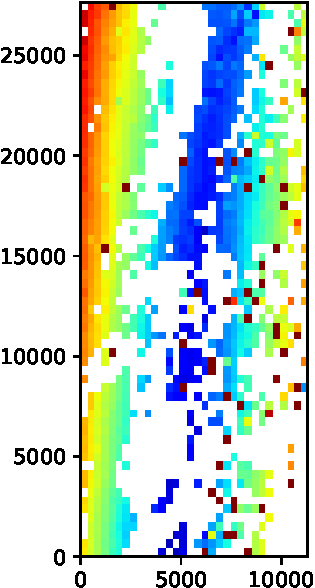
\includegraphics[width=0.8\textwidth]{xcorr-result}
    \end{minipage}
}
\subfloat[xcorr2]{
    \label{fig:exp_xcorr2_result}
    \begin{minipage}[t]{0.30\textwidth}
        \centering
        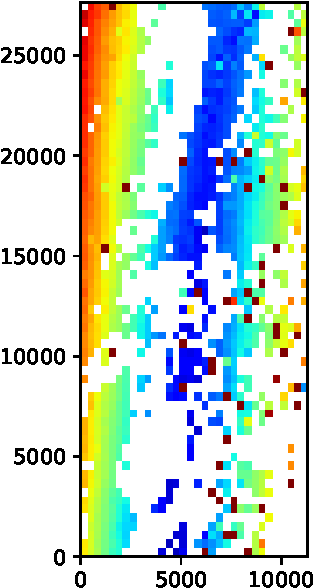
\includegraphics[width=0.8\textwidth]{xcorr2-result}
    \end{minipage}
}
\subfloat[偏移矢量差值]{
    \label{fig:exp_diff_result}
    \begin{minipage}[t]{0.39\textwidth}
        \centering
        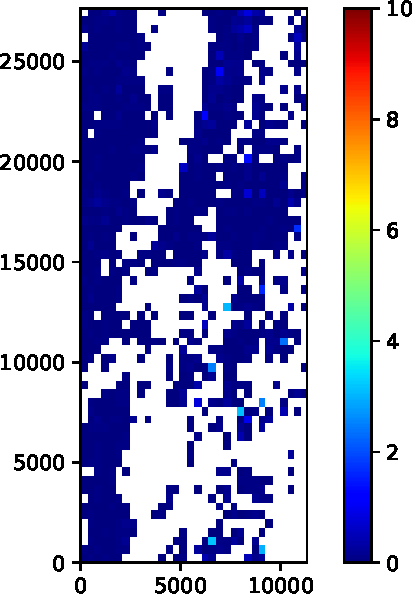
\includegraphics[width=0.8\textwidth]{diff-result}
    \end{minipage}
}
\caption{GMTSAR xcorr 与 xcorr2 配准结果对比} \label{fig:exp_result}
\note{\small 仅包含精配准偏移量。图中仅显示了偏移矢量长度,单位为像素。\\白色部分采样窗口最大互相关小于 GMTSAR aligh.csh 设定的最低值 18,因互相关性太差被筛除。}
\end{figure}

配准后 SLC 图像的相干性(公式 \ref{eq:coherence})是衡量配准精度的重要标准。图 \ref{fig:coh-two} 展示了分别经过 xcorr 和 xcorr2 配准后的主、副 SLC 图像相干性分布图,图 \ref{fig:coh-diff} 显示了相干性分布的差异。图像左下角部分,xcorr2 配准后的相干性略优,而左上角部分则反之。总体上看,相干性差异小于 $3 \times 10^{-3}$,几乎是可以忽略的。

\begin{figure}[htbp]
\centering
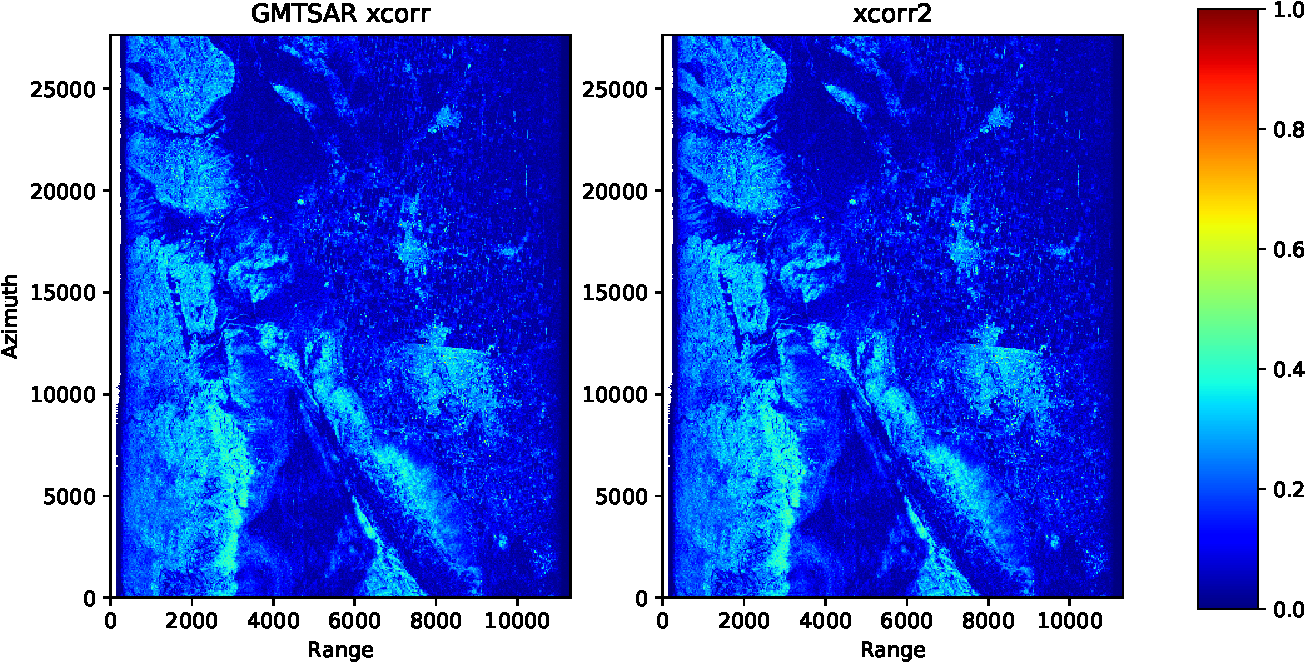
\includegraphics[width=0.85\textwidth]{coh-two}
\caption{配准后 SLC 图像相干性分布图} \label{fig:coh-two}
\note{\small 计算相干性时取像素周围 $8 \times 4$ 像素的邻域}
\end{figure}


\begin{figure}[htbp]
\centering
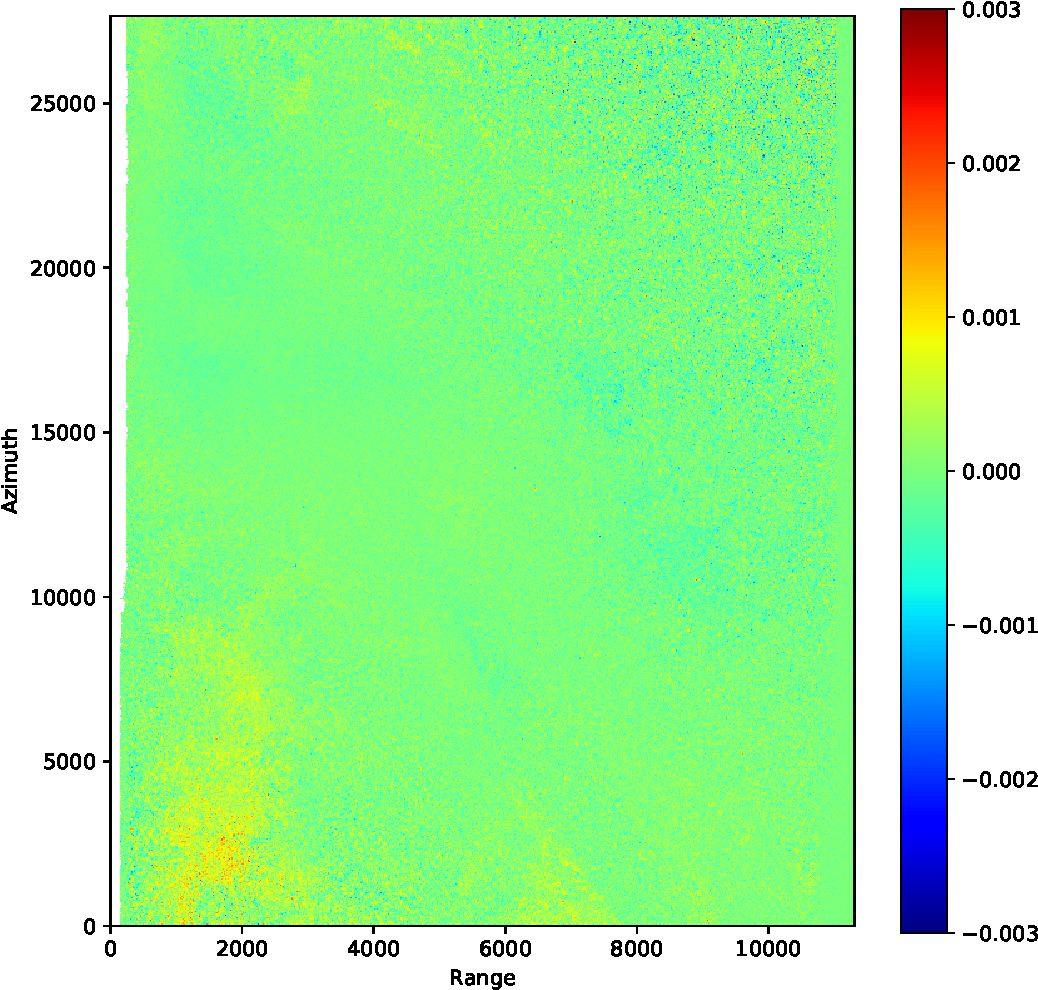
\includegraphics[width=0.60\textwidth]{coh-diff}
\caption{两幅相干性分布图的差值} \label{fig:coh-diff}
\note{\small 用 xcorr2 的计算结果减去 GMTSAR xcorr 的结果}
\end{figure}

\chapter{总结与展望}

\section{工作总结}

本课题对开源 InSAR 数据处理软件 GMTSAR 中的图像配准模块、图像拼接模块进行了并行优化,以提高桌面多核心 CPU 处理器上 InSAR 数据处理的效率。在真实 SAR 数据上进行的实验显示,并行程序在保证程序正确性的前提下大幅缩短了数据处理时间。

本课题基于 GMTSAR 图像配准模块 xcorr,设计了并行图像配准程序 xcorr2。基于硬件环境的定性分析,xcorr2 采用主-副多线程并行结构,使用一个主线程进行文件读取和线程管理,主线程以采样窗口为单位将配准任务分派给计算线程处理。此外,xcorr2 程序还对算法中部分 FFT 算法进行了简化,如使用实序列 FFT 算法代替复序列 FFT 算法。实验对比显示,xcorr2 在不影响配准精度的前提下通过多线程并行显著缩短了配准算法执行时间、提高了多核心 CPU 利用率。

本课题还设计了并行图像拼接程序。图像拼接程序利用并行优化中常用的规约技术,将拼接任务进行多线程分治并多层迭代拼接得到结果。在实验测试中,并行规约技术将图像拼接程序执行时间降低了一半以上。

受课题时间与个人能力限制,本课题仅完成 GMTSAR 软件中部分模块的优化工作。为了弥补这一不足,本文对干涉图生成、相位解缠等其他模块的并行优化进行了简单的讨论和分析,希望今后能够继续完成这些未尽的工作。

\section{未来展望}



\bibliography{bib/tex}

\appendix
\backmatter
\begin{acknowledgements}

中国科大地球和空间科学学院查显杰副教授,作为本课题指导老师,在课题实施中给予了充分的指导和帮助。其课题组的同学们也提出了很多宝贵的意见。感谢查老师和同学们的悉心指导和帮助。

实验测试是在中科院电磁空间信息重点实验室张卫明教授课题组的 Linux 计算集群上进行的。感谢张老师课题组对课题的支持。

\end{acknowledgements}


\end{document}
